\begin{figure}
\centering
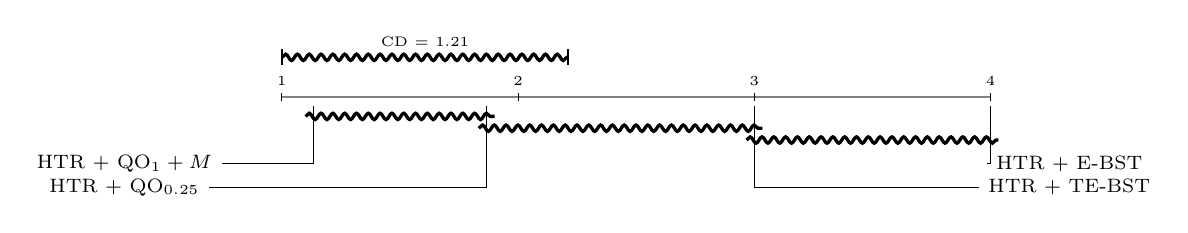
\begin{tikzpicture}[xscale=2]
\node (Label) at (2.40827866043412, 0.7){\tiny{CD = 1.21}}; % the label
\draw[decorate,decoration={snake,amplitude=.4mm,segment length=1.5mm,post length=0mm},very thick, color = black] (1.5,0.5) -- (3.3165573208682404,0.5);
\foreach \x in {1.5, 3.3165573208682404} \draw[thick,color = black] (\x, 0.4) -- (\x, 0.6);
 
\draw[gray, thick](1.5,0) -- (6.0,0);
\foreach \x in {1.5,3.0,4.5,6.0} \draw (\x cm,1.5pt) -- (\x cm, -1.5pt);
\node (Label) at (1.5,0.2){\tiny{1}};
\node (Label) at (3.0,0.2){\tiny{2}};
\node (Label) at (4.5,0.2){\tiny{3}};
\node (Label) at (6.0,0.2){\tiny{4}};
\draw[decorate,decoration={snake,amplitude=.4mm,segment length=1.5mm,post length=0mm},very thick, color = black](1.65,-0.25) -- (2.8499999999999996,-0.25);
\draw[decorate,decoration={snake,amplitude=.4mm,segment length=1.5mm,post length=0mm},very thick, color = black](2.75,-0.4) -- (4.55,-0.4);
\draw[decorate,decoration={snake,amplitude=.4mm,segment length=1.5mm,post length=0mm},very thick, color = black](4.45,-0.55) -- (6.05,-0.55);
\node (Point) at (1.7, 0){};\node (Label) at (0.5,-0.8500000000000001){\scriptsize{HTR + QO$_{1} + M$}}; \draw (Point) |- (Label);
\node (Point) at (2.8, 0){};\node (Label) at (0.5,-1.1500000000000001){\scriptsize{HTR + QO$_{0.25}$}}; \draw (Point) |- (Label);
\node (Point) at (6.0, 0){};\node (Label) at (6.5,-0.8500000000000001){\scriptsize{HTR + E-BST}}; \draw (Point) |- (Label);
\node (Point) at (4.5, 0){};\node (Label) at (6.5,-1.1500000000000001){\scriptsize{HTR + TE-BST}}; \draw (Point) |- (Label);
\end{tikzpicture}
\caption{Nemenyi - htr memory.csv}
\label{fig:nemenyi}
\end{figure}
